%\def\newblock{\hskip .11em plus .33em minus .07em}

\documentclass{llncs}
\usepackage{graphicx}
\sloppy

\usepackage{amssymb}
\usepackage{amsmath}
\usepackage{graphicx}
\usepackage{epsfig}
\usepackage{subfigure}
\usepackage{listings}
\usepackage{verbatim}
\usepackage[T1]{fontenc} 
\usepackage{url}
\lstset{language=ml}
\lstset{commentstyle=\textit}
\lstset{mathescape=true}
\lstset{backgroundcolor=,rulecolor=}
\lstset{frame=single}
\lstset{breaklines=true}
\lstset{basicstyle=\ttfamily \small}

\newcommand{\Nat}{{\mathbb N}}
\newcommand{\Real}{{\mathbb R}}

\begin{document}

\title{Monadic Scripting in F\# for Computer Games}

\author{
G. Maggiore, \ M. Bugliesi, \ R. Orsini
  \institute{Universit\`a Ca' Foscari Venezia \\
  \email{\{maggiore,bugliesi,orsini\}@dais.unive.it}
}
}

\maketitle

\date{}

\begin{abstract}
Modern game architectures provide for a clean separation between
game engine and game content, making engines \textit{scriptable}, so
as to delegate the development of the main functionalities related to
gameplay to scripts coded in high-level languages. 

Game scripting poses two orders of problems. First, the scripting
language must be equipped with coroutining mechanisms to support a
smooth interaction between the discrete-time structure of the game
animation implemented by the engine with the execution of the
scripts, which typically implement character behavior spanning 
multiple simulation ticks. Secondly, these mechanisms should be transparent, to
ease design and development, and at the same time offer the highest
run-time performance to keep up with the interactive frameratess
expected by the user. 

We present a monadic framework that elegantly solves these problems
and compare it with the most commonly used systems, and discuss how it has
been integrated in actual projects. 
\end{abstract}

\keywords{games, monadic programming, state management, scripting}

\section{Introduction}
\label{sec:intro}
%%%%%%%%%%%%%%%%%%%%%%%%%%%%%%%%%%%%%%%%%%%%%%%%%%%%%%%%%%
% intro.tex
%%%%%%%%%%%%%%%%%%%%%%%%%%%%%%%%%%%%%%%%%%%%%%%%%%%%%%%%%%

Game are:
- complex
- require performance

Low-level languages do not cut it fully.

We will:
(A) discuss game constraints
  - discuss traditional approaches and their limitations
  - discuss similarities between game genres and try and find a general framework
  - define a language that is built around this general framework, and which makes it easy
  - reason on why we'd rather have a new language and not just a library
  - give syntax, typing, semantics
(B) give optimization transformations of the language
(C) give a detailed case study
  - give benchmarks that show how effective our optimizations are and how they are completely automated (they require no effort on the part of the programmer) 
% 0 pages

\section{Game Engine Architectures}
\label{sec:scripting_in_games}
%%%%%%%%%%%%%%%%%%%%%%%%%%%%%%%%%%%%%%%%%%%%%%%%%%%%%%%%%%
% scripting_in_games.tex
%%%%%%%%%%%%%%%%%%%%%%%%%%%%%%%%%%%%%%%%%%%%%%%%%%%%%%%%%%

In this section we briefly illustrate a (heavily) simplified game architecture in order to describe the main problems that a scripting system faces when introduced inside a game engine.

A game engine is based on three fundamental components: 
({\em i}) the game state, which is a snapshot of the game world
and includes a description of all the various entities of the game; 
({\em ii}) the update  function, which computes the next value of the
game state, and ({\em iii}) the draw/rendering function, which draws
the game state to the screen.

The game loop is the code that defines how the game is run; it is a
recursive function that continuously invokes the update and draw
functions with the current state as input. The game loop also computes
the time delta between iterations, so that the update function will be
able to adjust its computations to cover the actual amount of time
elapsed between its invocations: 

\begin{lstlisting}
let run_game (game:Game) t =
  let t' = get_time()
  do game.Update (game.State, t'-t, t)
  do game.Draw (game.State)
  do run_game game t'
\end{lstlisting}

Central to our present concerns is the update function, which
implements all the functionalities that modify the game state. As 
discussed earlier, most of these functionalities, typically the
physics of the various entities, such as forces, 
collision detection, $\dots$ etc, the interaction with the
input/output and other devices are coded in low-level languages such
as C or C++ to guarantee the fast framerates  needed for a smooth play
experience. On the other hand, higher-level aspects of the game,
related to gameplay, are typically left outside the code of the 
update function, and made scriptable.  

The most important function of the scripts is to model the behaviors
of the computer characters and of the other in-game objects. To
illustrate, the following pseudo-code describes the behavior of  
a prince in a Role Playing Game: 

\begin{lstlisting}
prince:
  princess = find_nearest_princess()
  walk_to(princess)
  save(princess)
  take_to_castle(princess)
\end{lstlisting}

The main problem in coding this behavior with a script is to achieve a
smooth interaction between the discrete-time structure of the game
animation implemented by the simulation engine, and the behavior
implemented by the script, which spans multiple time slots of the
simulation engine. Specifically, in order to guarantee a smooth user
experience, each such script must be interruptible, so that at 
each discrete step of the simulation engine the script performs a
finite number of transitions and then suspend itself: failing to do 
so would slow down the simulation steps, hence the resulting framerate
of the game would decrease, thereby reducing the player immersion. 

The problem is sometimes addressed by coding scripts as state machines
(SMs), whose execution gets interrupted at each state transition. 
However, while SMs represent a viable design choice for simple
scripts, they are far less effective for modelling objects with
complex behavior, as their structure grows easily out of control and
becomes rather hard to maintain. Modern scripting languages adopt 
\textit{coroutines} as a mechanism to build state machines
implicitly, by way of their (the coroutines') built-in mechanisms to
suspend and resume execution. With coroutines the 
code for a SM is written ``linearly'' one statement after another, but
each action may suspend itself (an operation often called ``yield'')
many times before completing. The local state of the state machine
is stored in the continuation of the coroutine. Some of the most used 
scripting languages, which are Lua, Python and C\#, all offer some
suspension mechanisms similar to coroutines that game developers use
for scripting; for a detailed discussion of couroutines in these
languages, see \cite{PYTHON_COROUTINES,LUA_COROUTINES,CSHARP_YIELD}. 

\begin{comment}
\subsection{Coroutines in action}
In the remainder of this section we analyze coroutines in action in Lua. We will also briefly discuss how coroutines are emulated in Python and C\# with generators. For a more detailed discussion of the mechanisms of coroutines in Lua, Python and C\# see \cite{PYTHON_COROUTINES,LUA_COROUTINES,CSHARP_YIELD}.

Lua coroutines are based on the three functions \texttt{coroutine.yield, coroutine.resume} and \texttt{coroutine.create} which respectively pause execution of a coroutine, resume execution of a paused coroutine and create a coroutine from a function.

\begin{lstlisting}
function walk_to(self,target)
  return coroutine.create(
    function()
      while(dist(self,target) > self.reach) do
        self.Velocity = towards(self, target)
        coroutine.yield()
      end
    end)
end

...

function prince(self)
  return coroutine.create(
    function()
      princess = bind_co(find_nearest_princess(self))
      bind_co(walk_to(self, princess))
      bind_co(save(self, princess))
      bind_co(take_to_castle(self, princess))
    end)
end
\end{lstlisting}

Notice that to invoke a coroutine we need to explicitly bind it with the \texttt{bind\_co} function (we do not show here the source for reasons of space), which keeps resuming a coroutine until it yields for the last time, and then it returns the resulting value.

A mechanism to implement coroutines in Python makes use of generators. A generator is a special routine that returns a sequence of values. However, instead of building an array containing all the values and returning them all at once, a generator yields the values one at a time; yielding effectively suspends the execution of the generator until the next element of the sequence is requested by the caller. Python generators may appear as a way to return lazy sequences but they are powerful enough to implement coroutines. We can adopt the convention that a coroutine is actually a generator which yields a sequence of null (\texttt{None}) values until it is ready to return; the returned value will be yielded last.

\begin{lstlisting}
def walk_to(self,target):
  while(dist(self,target) > self.Reach):
    self.Velocity = towards(self,target)
    yield

...

def prince(self):
  for princess in find_nearest_princess(self):
    yield
  for x in walk_to(self,princess):
    yield
  for x in save(self,princess):
    yield
  for x in take_to_castle(self,princess):
    yield
\end{lstlisting}

As in Python, C\# supports generators. Since C\# is statically typed, we need to assign a type to our coroutines. We have two alternatives; a coroutine that returns nothing (\texttt{void}) has type \texttt{IEnumerable}, that is it returns a sequence of \texttt{Object}s that are all null (a similar strategy is used by Unity, even though with unsafe casts \cite{UNITY_YIELD}) and we can type a coroutine that returns a value of type \texttt{T} as \texttt{IEnumerable<T?>}, where \texttt{T?} is either \texttt{null} or an instance of \texttt{T}.

We omit the C\# sample for brevity, and also because of its similarity with Python. Moreover, when compared with coroutines, generators are quite cumbersome in a scripting language and indeed LUA is by far more used in games.

In the remainder of the paper we will present a different approach to coroutines, namely building a meta-programming abstraction (called \textit{monad}) to implement coroutines in F\#. We will discuss how our approach produces code which is faster and shorter than similar implementations in Lua, Python and C\#. We will also discuss how our approach is very customizable, thanks to the fact that coroutines are not \textit{wired} into the language runtime but rather we have defined them with our monad. Monads simplify the use of coroutines, making them completely invisibile to the user. Also, thanks to type inference the resulting scripts require no typing annotations. 
Finally (see Section \ref{sec:benchmarks} for the details), our system offers a good runtime performance and is type safe; this makes it suitable for large and complex scripts.
\end{comment}
 
% 6 pages

\section{The Script Monad}
\label{sec:script_monad}
%%%%%%%%%%%%%%%%%%%%%%%%%%%%%%%%%%%%%%%%%%%%%%%%%%%%%%%%%%
% script_monad.tex
%%%%%%%%%%%%%%%%%%%%%%%%%%%%%%%%%%%%%%%%%%%%%%%%%%%%%%%%%%

Monads can be used for many purposes \cite{MOGGI_MON,DECL_IMP,COMPR_MON,EFF_MON,CSHARP_ASYNC,CSHARP_LINQ}. Indeed, monads allow us to
overload the bind operator, in order to define exactly what happens
when we bind an expression to a name.  We will use this capability of monads to implement a DSL for coroutines that allows to chain coroutines together with the binding operator. The monad we define will \textit{suspend} itself at every bind and return its continuation as a lambda. The monad type is \texttt{Script}: 

\begin{lstlisting}
type Script<'a,'s> = 's -> Step<'a,'s>
 and Step<'a,'s> = Done of 'a | Next of Script<'a,'s>
\end{lstlisting}

Notice that the signature is very similar to that of the regular
state monad, but rather than returning a result of type $\alpha$
it returns either \texttt{Done\ of} $\alpha$ or the continuation 
\texttt{Next\ of\ Script<}$\alpha,\sigma$\texttt{>}. The continuation stores, in its closure, the local state of a suspended script. Our monad allows us to access the state which will be passed by the game engine; this way our scripts will be able to read, write or modify the main state of the game to interact with the processing performed by the game engine.

Returning a result in this monad is simple: we just wrap it in the
$\mathtt{Done}$ constructor since obtaining this value  requires no
actual computation steps. Binding together two statements is more complex. 
We try executing the first statement; if the result is
$\mathtt{Done\ x}$, then we return
$\mathtt{k\ x\ s}$, that is we perform the binding and we 
continue with the rest of the program with the result of the first
statement plugged in it. If the result is \texttt{Next\ p'}, then we cannot
yet invoke $\mathtt{k}$. This means
that we have to bind \texttt{p'} to \texttt{k}, so that at the next
execution step we will continue the execution of \texttt{p} from where
it stopped.

\begin{lstlisting}
type ScriptBuilder() = 
  member this.Bind(p:Script<'a,'s>, k:'a->Script<'b,'s>) 
    : Script<'b,'s> =
    fun s ->
      match p s with
      | Done x -> k x s
      | Next p' -> Next(this.Bind(p',k))

  member this.Return(x:'a) : Script<'a,'s> = fun s -> Done x

let script = ScriptBuilder()
\end{lstlisting}

We now define the \texttt{get\_state} coroutine that extracts the current state:

\begin{lstlisting}
let get_state : Script<'s,'s> = fun s -> Done s
\end{lstlisting}

We also define another coroutine that forces a suspension:

\begin{lstlisting}
let suspend :Script<Unit,'s> = fun s -> Next(fun s -> Done())
\end{lstlisting}

We assume the standard F\# convention that \texttt{let! x = script1 in script2} is translated into \texttt{Bind(script1, fun x -> script2)} and \texttt{return x} is translated into \texttt{Return(x)}.

Let us now see a small, self-contained example of our scripting system in action. Coroutines can be used in many ways to achieve various results; what we are more interested in, is using coroutines as a means to perform long and complex computations asynchronously inside the main loop of an application. We wish to build an application that computes a very large Fibonacci number, but does so while continuously writing on the console that it is still alive and responsive. This application has no shared state, and so all our coroutines will have type \texttt{Script<'a,Unit>}.

The coroutine version of the Fibonacci function is very similar to a regular implementation of the Fibonacci function, with the only difference that we use monadic binding to recursively invoke the function itself. Each time we recurse, the coroutine suspends:

\begin{lstlisting}
let rec fibonacci n : Script<int,Unit> = 
  script{
    match n with
    | 0 -> return 0
    | 1 -> return 1
    | n -> 
      do! suspend
      let! n1 = fibonacci (n-1)
      let! n2 = fibonacci (n-2)
      return n1+n2 
  }
\end{lstlisting}

Running the Fibonacci function now requires many steps of our scripting monad; for this reason we can safely invoke this function with the knowledge that it will run for a short time before returning either the final result with \texttt{Done} or its continuation with \texttt{Next}. We can define the main loop of our application as follows:

\begin{lstlisting}
let main_loop() =
  let rec main_loop (f:Script<int,Unit>) = 
    do printf "I am alive.\n"
    match f () with
    | Done result -> 
      do printf "The result is %d\n" result
    | Next f' ->
      main_loop f'
  do main_loop (fibonacci 1000000) 
\end{lstlisting}

The main loop above can be seen as a simplification of the game loop we have seen in Section \ref{sec:intro}. Of course in a game the state datatype would be more complex than just \texttt{Unit}, and the application would perform its full update and draw instead of just printing a string on the screen. This said, adding the above pattern matching to each iteration of the main loop of the game is all that is required to integrate our scripting system with an existing game engine.

 
% 3 pages

\section{A DSL for Scripting}
\label{sec:script_combinators}
%%%%%%%%%%%%%%%%%%%%%%%%%%%%%%%%%%%%%%%%%%%%%%%%%%%%%%%%%%
% script_monad_combinators.tex
%%%%%%%%%%%%%%%%%%%%%%%%%%%%%%%%%%%%%%%%%%%%%%%%%%%%%%%%%%

The script monad is the runtime core of our DSL. A DSL can be augmented by defining a series of operators that automate or simplify common operations for the DSL developers. The best set of operators for a scripting DSL is strongly dependent upon the kind of game to be scripted. In this section we describe a general-purpose set of operators that make up a basic calculus of coroutines, but we would expect that other game developers would define additional operators that are a tighter fit to their games. The operators of our calculus of coroutines take as input one or more coroutines and return as output a new coroutine:

\begin{itemize}
\item \texttt{parallel} ($s_1 \wedge s_2$) executes two scripts in parallel and returns both results
\item \texttt{concurrent} ($s_1 \vee s_2$) executes two scripts concurrently and returns the result of the first to terminate
\item \texttt{guard} ($s_1 \Rightarrow s_2$) executes and returns the result of a script only when another script evaluates to \texttt{true}
\item \texttt{repeat} ($\uparrow s$) keeps executing a script over and over
\item \texttt{atomic} ($\downarrow s$) forces a script to run in a single tick of the \textit{discrete simulation engine}
\end{itemize}

We show here the implementation of one of these combinators with our monadic system. To see the other implementations, see \cite{FRIENDLY_FSHARP}.

\begin{lstlisting}
let rec parallel_ (s1:Script<'a>) (s2:Script<'b>) 
          : Script<'a * 'b> =
  fun s ->
    match s1 s,s2 s with
    | Done x, Done y    -> Done (x,y)
    | Next k1, Next k2  -> parallel_ k1 k2
    | Next k1, Done y   -> parallel_ k1 (fun s -> Done y)
    | Done x, Next k2   -> parallel_ (fun s -> Done x) k2
\end{lstlisting}


We can now give another self-contained example that shows a producer and a consumer running in parallel. We start by defining the state as a single memory location, which can either be empty (\texttt{None}) or contain a value (\texttt{Some x}):

\begin{lstlisting}
type Buffer = { mutable Contents : Option<int> }
let buffer = { Contents = None }
\end{lstlisting}

We define some additional helper functions to access the state. A good engineering rule is that the more complex is the state, the less coroutines directly use the \texttt{get\_state} function; rather, when the state is complex, we define a series of additional accessor functions that help us manipulating the various aspects of the state:

\begin{lstlisting}
let set_buffer v : Script<Unit,Buffer> = 
  script{
    let! s = get_state
    s.Contents <- Some v }
let is_buffer_empty : Script<bool,Buffer> = 
  script{
    let! s = get_state
    return s.Contents = None }
\end{lstlisting}

We define the producer (the consumer is symmetric) as follows; notice that each access to the state automatically suspends the coroutine, so we do not need to explicitly invoke \texttt{suspend}:

\begin{lstlisting}
let rec wait_buffer_empty:Script<Unit,Buffer> = 
  script{
    let! c = is_buffer_empty
    if c = false then
      do! suspend
      do! wait_buffer_empty }

let producer =
  let rec producer i : Script<Unit,Buffer> =
    script{
      do! wait_buffer_empty
      do! set_buffer i
      do! producer (i+1) }
\end{lstlisting}

The main loop is very similar to the main loop seen for the Fibonacci sample above; the only difference is that we invoke the producer and the consumer coroutines in parallel, by passing to the inner \texttt{main\_loop} function the value \texttt{parallel\_ producer consumer}.


\subsection{Scripting in Games}

We now discuss the introduction of our scripting system in games. In the following we outline how we have built most of the game logic of the upcoming RTS game Galaxy Wars (which is also released with a fully open source \cite{GALAXY_WARS}). In the game we are considering the players compete to conquer a series of \textit{star systems} by sending fleets to reinforce their systems or to conquer the opponent's.

\subsubsection{Game Patterns}

Thanks to our general combinators we can define a small set of recurring game patterns; by instantiating these game patterns one can build the actual game scripts with great ease. These patterns may be adapted for the specific domain of a game, or altogether new patterns may be created that better fit one's game. 
The first game pattern we see is the most general, and for this reason it is called \texttt{game\_pattern}. This pattern initializes the game in a single tick, then performs a game logic (while the game is not over) and finally it performs the ending operation before returning some result. The initialization is performed by the \texttt{init} script, which returns a result of a generic type \texttt{'a}; this result is the state of the script, and contains data that may be helpful for tracking additional information that is useful to our scripts but which is not stored in the game state. The logic of the various game entities, such as their AI, is then performed, repeatedly, by the \texttt{logic} script. While the logic script is run, the \texttt{game\_over} script continuously checks to see if the game has been won or lost and thus must be terminated; when the termination condition is met, the \texttt{ending} script is invoked that may show some recap of the game that has just ended. The game pattern is implemented as follows:

\begin{lstlisting}
let game_pattern 
      (init:Script<'a>) 
      (game_over:'a -> Script<'bool>) 
      (logic:'a -> Script<Unit>) 
      (ending:'a -> Script<'c>) 
      : Script<'c> =
  script{
    let! x = init |> atomic_
    let! (Left y) = 
       concurrent_ 
         (guard_ (game_over x) (ending x)) 
         (logic x |> repeat_)
    return y }
\end{lstlisting}

Notice that with the introduction of appropriate operators we may remove many of the parentheses of the above sample if they are seen as a hindrance to readability. The main portion of the code above may then be rewritten as:

\begin{lstlisting}
(game_over x => ending x) .|| (logic x |> repeat_)
\end{lstlisting}

The game pattern above is very general, but not all scripts always need all of its parameters. We can build less general game patterns by reducing the number of parameters; for example, we may build a game pattern that has no initialization, logic or ending sequence; such a game pattern would implement the case of a game script whose sole responsibility is to check the termination conditions for a game (those that trigger the ``game over'' screen):

\begin{lstlisting}
let wait_game_over (game_over:Script<bool>) : Script<Unit> = 
  let null_script = script{ return () }
  game_pattern 
    null_script
    (fun () -> game_over)
    (fun () -> null_script)
    (fun () -> null_script)
\end{lstlisting}

Writing a script with our system will consist of instantiating one game pattern with specialized scripts as its parameters; these scripts will alternate accesses to the specific state of the game with invocations of combinators from the calculus seen above. In the next session we will see an example of this.
 
% 5 pages

\label{sec:script_monad_case_study}
%%%%%%%%%%%%%%%%%%%%%%%%%%%%%%%%%%%%%%%%%%%%%%%%%%%%%%%%%%
% script_monad_case_study.tex
%%%%%%%%%%%%%%%%%%%%%%%%%%%%%%%%%%%%%%%%%%%%%%%%%%%%%%%%%%

\subsubsection{A sample script}

The state of the game contains a series of star systems, fleets, players and various other information:

\begin{lstlisting}
type GameState = {
    StarSystems : StarSystem List
    Fleets      : Fleet List
    ... }
\end{lstlisting}

We define a series of accessor functions that allow a coroutine to access the current state of the game; such an accessor function, for example, is the \texttt{get\_fleets} that returns the list of active fleets:

\begin{lstlisting}
let get_fleets = 
  script{
    let! state = get_state
    return state.Fleets }
\end{lstlisting}

The basic mode of the game uses our scripting system to determine the winner of the game; as long as there is more than one player standing, the script waits. This script computes the union of the set of active fleet owners with the set of system owners:  

\begin{lstlisting}
let alive_players_set = 
  script{
    let! fs = get_fleets
    let fleet_owners = 
             fs |> Seq.map (fun f -> f.Owner) 
             |> Set.ofSeq
    let! ss = get_systems
    let system_owners = 
             ss |> Seq.map (fun s -> s.Owner) 
             |> Set.ofSeq
    return fleet_owners + system_owners }

let game_over =
  script{
    let! alive_players = alive_players_set
    let num_alive_players = alive_players |> Seq.length
    return num_alive_players = 1 }
\end{lstlisting}

The main task of our script is to wait until the set of active players has exactly one element; when this happens, that player is returned as the winner: 

\begin{lstlisting}
let basic_game_mode = wait_game_over game_over
\end{lstlisting}

The two short snippets above are all there is to the main game mode.

Variations of the game are soccer (one system acts as the ball which can be moved around), capture the flag, siege and others. We omit a detailed discussion of the other variations for reasons of space; the important thing to realize is that all of these variations have been implemented with the same simplicity of the scripts above, by instancing one game pattern with appropriate scripts which are built with a mix of combinators interspersed with accesses to the game state.

\subsubsection{Input Management}

Another large subsystem where we have used our scripting system is input management. Input is divided into a series of pairs of scripts; each pair of scripts is separated by a guard: the first script performs an event detection, while the second performs an event response. Each pair of scripts is repeated forever, in parallel with all other scripts.

As an example, consider the following script that decides whether to launch ships or not against a target:
\begin{lstlisting}
let input world = 
  repeat_(
  script{ 
    if mouse_clicked_left() then
      let mouse = mouse_position()
      // find closest planet under the cursor
      let clicked:Option<Planet> = ... 
      return Some(clicked) } => 
    fun p -> script{ world.SourcePlanet := Some(p) }) .||
  repeat_(
  script{ 
    if mouse_clicked_right() && 
       world.SourcePlanet <> None then
      let mouse = mouse_position()
      // find closest planet under the cursor
      let clicked:Option<Planet> = ... 
      match clicked with 
      | Some planet -> 
        return Some(planet,world.SourcePlanet.Value)
      | None -> return None } => 
    fun (source,target) -> 
      script{ mk_fleet world source target })
\end{lstlisting}

A distinct advantage of this technique is that it allows us to cleanly separate the code that reads the actual user input from the code that performs something meaningful on the game world with this input. By parametrizing the code above with respect to the input detection scripts we could make it possible to support different controller types (game pad, touch panel, mouse, keyboard, etc.).

\subsubsection{Further uses}

Since our scripting system proved effective in the various areas where we tried it, and given that its performance is fully satisfactory, we have decided to use it more pervasively all over the game. The result is that each entity (planets, ships, players, etc.) has a large chunk of its game logic moved from the update loop into appropriate scripts.

Our menu system is heavily based on our scripts (this proved especially useful when implementing the multi-player lobby, where the regular menu (buttons, input detection, etc.) had to be run interleaved with the scripts that synchronize the list of players across the network.

Finally, we have used scripts for the entire networking system, given that many operations such as connections and time-outs require timers and many parallel operations. 
% 2 pages

\section{Benchmarks}
\label{sec:benchmarks}
%%%%%%%%%%%%%%%%%%%%%%%%%%%%%%%%%%%%%%%%%%%%%
% BENCHMARKS
%%%%%%%%%%%%%%%%%%%%%%%%%%%%%%%%%%%%%%%%%%%%%

- Windows, Xbox, Wp7 (, iPad?)
- memory recycling
- parallel execution
- query optimization
 
% 2 pages

\section{A Visual Editor (future work)}
\label{sec:visual_editor}
%%%%%%%%%%%%%%%%%%%%%%%%%%%%%%%%%%%%%%%%%%%%%%%%%%%%%%%%%%
% future work
%%%%%%%%%%%%%%%%%%%%%%%%%%%%%%%%%%%%%%%%%%%%%%%%%%%%%%%%%%

One of our main concerns is that our scripting system as presented so far is aimed at technical users. While this definitely offers advantages, since the game engine itself can be partially coded with scripts to the great benefit of the productivity of developers, the need for less technically inclined users such as designers to access the scripting system is very relevant. After all, designers play a very important role in shaping the behaviors and scripts of a game.

For this reason we are studying a visual editor that allows to create scripts without having to write source code. This editor (which is still a work in progress) would allow the user to drag blocks that represent operations and combinators of our scripts, and assemble them in a fashion that is similar to that of flow-charts.

One of the scripts that we have seen above:

\begin{lstlisting}
(game_over x => ending x) .|| (logic x |> repeat_)
\end{lstlisting}

Would appear in our editor as:

\begin{center}
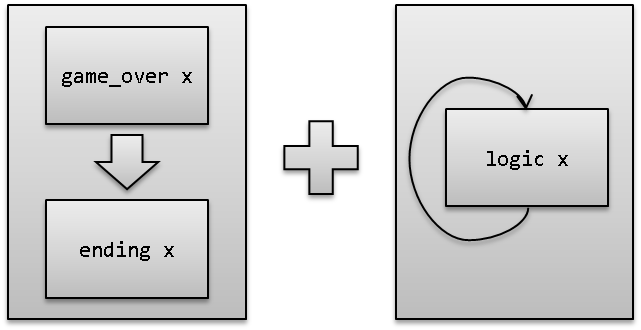
\includegraphics[scale=0.5]{visual_script.png}
\label{Visual script}
\end{center}
 

\section{Conclusions}
\label{sec:conclusions}
%% Changed by PS, April 4, 2014.

\section{Future work}
\label{sec:future_work}
The Casanova 2 language is capable of implementing usable and quite complex games. The language, while usable, is currently still in development as it misses a few features. In particular, support for multiplayer games is at this moment lacking. We believe that the existing mechanisms for handling time offered by Casanova 2 could be augmented with relatively little effort in order to greatly simplify the hard task of building multiplayer games. This is part of future work, that we are currently engaging in. We are also doing usability studies using students from various disciplines and backgrounds.

The high level view of the game that the Casanova 2 compiler provides can be exploited in order to improve the programmer experience. This means that we could use tools for code analysis (such as abstract interpretation \cite{nielson1999principles} or type system extensions) in order to better understand the game being built, and to help with correctness analysis, performance analysis, or even optimization.


%\subsection{User study}
%We wish to perform an in-depth user study for Casanova 2 to improve usability in the development process. We have already performed a partial (and quite promising) small user study which we will extend and complete.


%We have performed the following test: we gathered a group of students of game programming and a group of students of game design. We gave them a series of Casanova 2 samples, printed on paper. Each student had to guess the functionality of each sample, and sketch a screen-shot. Furthermore, each student also provided some additional feedback on the language.

%The samples were: (\textit{i}) a string of text moved around the screen with the keyboard, (\textit{ii}) a string of text that moves along a predefined path automatically, and (\textit{iii}) an asteroid shooter.

%Eleven (over a total of thirteen) students understood the samples completely, both drawing the screen-shots and explaining the dynamics of the game correctly. Two students were lost on the syntactic differences between Casanova 2 and the more familiar C-like syntax. The direct feedback was mostly centred around a series of common observations, which are reported in Table \ref{students_feedback}. For each observation, the table reports how many times we encountered it.

%\begin{table}[!t]
%% increase table row spacing, adjust to taste
%\renewcommand{\arraystretch}{1.3}
% if using array.sty, it might be a good idea to tweak the value of
% \extrarowheight as needed to properly center the text within the cells

%\caption{Feedback from students}
%\label{students_feedback}
%\centering

%% Some packages, such as MDW tools, offer better commands for making tables
%% than the plain LaTeX2e tabular which is used here.
%\begin{tabular}{|c||c|}
%\hline
%Syntax is unfamiliar at first & 3\\
%\hline
%Syntax is clear & 8\\
%\hline
%Indentation instead of parentheses is a downside & 2\\
%\hline
%List processing with queries is very effective & 1\\
%\hline
%Rules are a good abstraction for games & 2\\
%\hline
%\end{tabular}
%\end{table}

%We also built a significantly bigger sample, which we asked only three students to study. The sample is a checkpoint-based RTS (see Figure \ref{RTS game} for a screenshot). All students correctly identified the game mechanics, and provided some additional feedback. Most of this feedback overlaps with that obtained for the samples, but some new observations emerge. Arguably, some patterns become visible only with larger samples:
%\begin{itemize}
%\item \texttt{wait} and \texttt{when} are very powerful
%\item Multiple rules on the same field are very powerful
%\item Multiple rules on the same field may lead to behaviours that are complex to understand
%\end{itemize}


\section{Conclusions}
\label{sec:conclusions}

Casanova 2, a language specifically designed for building computer games, may offer a solution for the high development costs of games. The goal of Casanova 2 is to reduce the effort and complexities associated with building games. Casanova 2 manages the game world through entities and rules, and offers constructs (wait and yield) to deal with the run-time dynamics. As shown by the benchmarks in Section \ref{sec:evaluation}, we believe that we have taken a significant step towards reaching these goals. In fact, we achieved at the same time very good performance and simplicity, thereby empowering developers with limited resources.  
% 1 pages

\vfill\eject

\bibliographystyle{plain}
\bibliography{references} 
% 0 pages

\end{document}
